\section{Evaluering}

\subsubsection{Forskellige Operativsystemer}
For at sikre stabilitet af brugergrænsefladen er spillet afprøvet i forskellige størrelser og på forskellige operativsystemer. Placeringen af komponenterne er ens i Micrsoft Windows 8.1 og dens ældre versioner, iOS og Linux. Derimod har JButtons et lidt andet udseende på iOS, idet deres baggrundsfarve i dette operativsystem ikke er synlig medmindre deres kant skjules. Derudover virker de heller ikke for iOS, hvis de tilføjes til et panel i 'paintComponent'-metoden. Det første problem løses ved at skjule kanten eller i stedet at bruge et ImageIcon til knappen i stedet for at give den en baggrundsfarve. Knappens funktionalitet opnås ved at tilføje knapperne i konstuktøren, men 'setLocation'-metoden kan stadig ligge i 'paintComponent'-metoden for at give den samme effekt som tidligere. Vi havde i gruppen to personer med Windows, en med Linux og en med MAC.
\newline

Vi havde nogle problemer med lyden på Linux, idet spillet ikke spillede hele sekvensen fra lydfilerne, når spillet blev startet eller når spillet endte. Denne fejl har vi dog ikke kigget nærmere på, da der kan være rigtig mange fejlkilder. Det kan enten være Java implementeringen, at Linux er installeret forkert, lyd driveren eller andre hardware problemer.

\subsubsection{Køretid}
Efter tilføjelsen af en masse grafik og udvidede funktioner til Simple Snake, kunne man på nogle computere se at spillet ikke reagerede lige så hurtigt som før, og køretiden var for lang.
Dette ses især på en af vores sidste versioner af Advanced Snake, hvis man sætter størrelsen på banen til $100\times 100$. Man kunne ikke holde piletasterne nede, og få slangen til at køre hurtigere. Dette blev løst ved først at lave vores slange om fra billeder til filledRectangles igen, der fik spillet til at køre ved normal hastighed som før. 
For at få billederne til også at fungere ved normal hastighed, ændrede vi i stedet strukturen af hvornår billederne af slangens krop kalder 'getScaledInstance'-metoden. Tidligere blev hver del af slangen skaleret efter at være blevet udvalgt som den rigtige del igennem en for-løkke, mens alle billederne nu skaleres i forvejen, så billeder der bliver brugt flere gange, ikke behøver at skaleres hver gang. Dette løste problemet så køretiden igen var normal.

\subsubsection{Slangens farver}
Nederst i \textit{BoardBasePanel}-klassen ligger metoden \textit{colorSnakeImage}, som farver hver pixel i slange-billederne, så de passer med valgene fra menuen. 
Inden denne metode blev lavet, overvejede vi at importere fire gange så mange snake-billeder, som der oprindeligt var - til fire forskellige farver. Da det i forvejen er mange billeder, der bruges til slange-kroppen, ville dette være for mange billeder at importere, hvis man i stedet kunne finde en metode til farvningen.
På denne måde er farve-valg i menu'en blevet optimeret en del ved at bruge WritableRaster til farvningen.

\subsubsection{Knapper}
Da vi i starten ikke ville bruge JButtons på grund af deres design, var knapper i starten oprettet som tegnede rektangler med lige så store områder hvorpå man kunne klikke, hvilket ville give en illusion af en knap. Senere fandt vi ud af at JButtons kunne modificeres både med hensyn til udseende og størrelse. Dette gav dog problemer med vores oprindelige GridLayout i panelerne, idet knappen ville fylde hele dens felt i gitteret ud, og derved  blive for stor. Derfor endte vi med at bruge standard-layoutet FlowLayout og setLocation, der gjorde det let at manipulere med knappens placering i vinduet.

\begin{figure}[h]
	\centering
	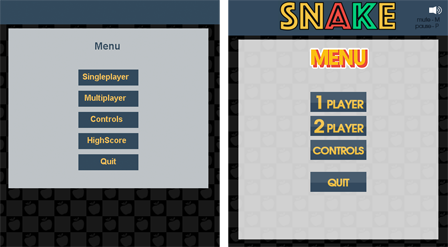
\includegraphics[width=0.8\textwidth]{Menu.png}
	\caption{\figlab{menu}\textit{Rektangler og JButtons}}
\end{figure}

\subsubsection{Implementering af multiplayer}
Ved implementeringen af multiplayer-spillet overvejede vi først at bruge en kombineret single- og multiplayer-klasse, som kunne holde et array af slanger. Hvis der var to slanger, ville vi bruge multiplayer-gameplay og singleplayer-gameplay ved én slange. Fordelen ved dette er, at view-delen i MVC-designet, bare kan loop over nogle arrays lige meget om det er single- eller multiplayer-spillet. Det vil være let at tjekke om spilleren er i singleplayer- eller multiplayer-spillet, da skal bare sættes et if-statement der tjekker for antallet af slanger. Det ville være nemt at tilføje flere slanger. Ulempen ved den fælles klasse er, at der vil være mange if-statements. At holde spillene adskilt gør det også lettere at lave justeringer i det ene spil uden at påvirke det andet. Der er ikke er klart overlegent valg, begge implementeringer har sine ulemper og fordele.